\clearpage

\section{SOP Modulator}

\begin{tcolorbox}	
\begin{tabular}{p{2.75cm} p{0.2cm} p{10.5cm}} 	
\textbf{Header File}   &:& SOP\_modulator\_20180319.h \\
\textbf{Source File}   &:& SOP\_modulator\_20180319.cpp \\
\textbf{Version}       &:& 20180319 (\textbf{Student Name}: Mariana Ramos)
\end{tabular}
\end{tcolorbox}


This block of code simulates a modulation of the State Of Polarization (SOP)in a quantum channel, which intends to insert possible errors occurred during the transmission due the polarization rotation of single photons. These SOP changes can be simulated using deterministic or stochastic methods. The type of simulation is one of the input parameters when the block is initialized.


\subsection*{Functional description}

This block intends to simulate SOP changes using deterministic and stochastic methods. The required function mode must be set when the block is initialized. Furthermore, other input parameters should be also set at initialization. If a deterministic method was set by the user, he also needs to set the $\theta$ and $\phi$ angles in degrees, which corresponds to the two parameters of Jones Space in Poincare Sphere thereby being the rotation and elevation angle, respectively.

\begin{figure}[h]
	\centering
	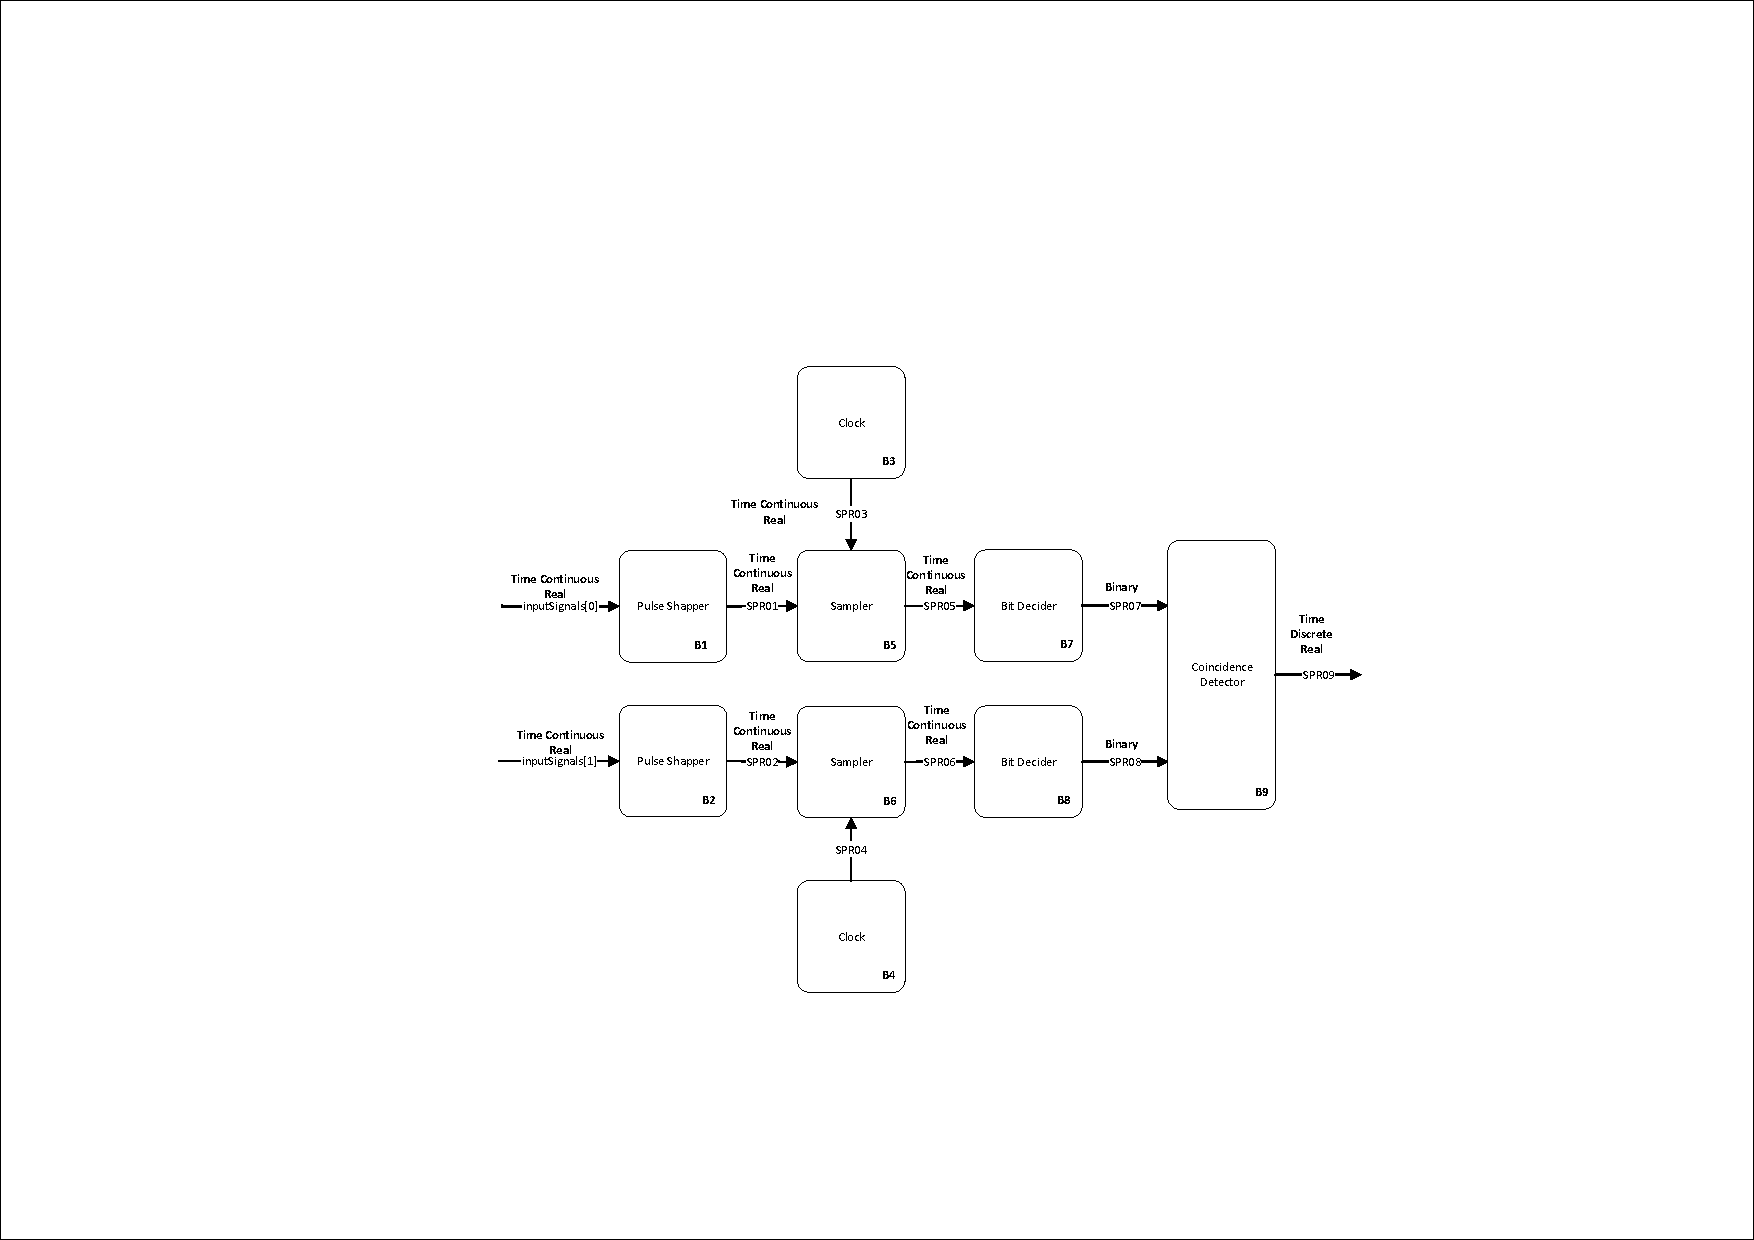
\includegraphics[clip, trim=8cm 4cm 6cm 5cm, width=1.00\textwidth]{../lib/single_photon_receiver/figures/single_photon_receiver.pdf}
	\caption{Basic configuration of the SPR receiver}\label{SPR_receiver_block_diagram_simple}
\end{figure}

SOP modulator block can have an input signal of a clock in order to achieve additional synchronization. However, it also works without an external clock and in this case it outputs a value of $\theta$ and $\phi$ continuously.


\subsection*{Input parameters}

SOP modulator block must have an input signals to set the clock of the operations. This block has some input parameters that can be manipulated by the user in order to change the basic configuration of the SOP modulator. Each parameter has associated a function that allows for its change. In the following table (table~\ref{table:sopmodulator_in_par}) the input parameters and corresponding functions are summarized.

\begin{table}[h]
	\centering
	\begin{tabular}{|c|c|c|c|cccc}
		\cline{1-4}
		\textbf{Parameter} & \textbf{Type} & \textbf{Values} &   \textbf{Default}& \\ \cline{1-4}
		sopType & SOPType & Deterministic or Stochastic & Deterministic \\ \cline{1-4}
		theta & double & any & 0.0 \\ \cline{1-4}
		phi & double & any & 0.0 \\ \cline{1-4}
	\end{tabular}
	\caption{List of input parameters of the block SOP modulator}
	\label{table:sopmodulator_in_par}
\end{table}


\subsection*{Methods}

SOPModulator(vector <Signal*> \&inputSignals, vector <Signal*> \&outputSignals)(\textbf\{constructor\})
\bigbreak
void initialize(void)
\bigbreak
bool runBlock(void)
\bigbreak
void setSOPType(SOPType sType)
\bigbreak
void setRotationAngle(double angle)
\bigbreak
void setElevationAngle(double angle)
\bigbreak



\subsection*{Input Signals}

\subparagraph*{Number:} 1

\subparagraph*{Type:} Time Continuous Amplitude Continuous Real (Clock)

\subsection*{Output Signals}

\subparagraph*{Number:} 2

\subparagraph*{Type:} Time Continuous Amplitude Discrete Real (correspond to the two parameters of Jones in units of degrees)

\subsection*{Example}

\subsection*{Sugestions for future improvement}
